\let\negmedspace\undefined
\let\negthickspace\undefined
\documentclass[journal]{IEEEtran}
\usepackage[a5paper, margin=10mm, onecolumn]{geometry}
\usepackage{tfrupee}

\setlength{\headheight}{1cm}
\setlength{\headsep}{0mm}

\usepackage{gvv-book}
\usepackage{gvv}
\usepackage{cite}
\usepackage{amsmath,amssymb,amsfonts,amsthm}
\usepackage{algorithmic}
\usepackage{graphicx}
\usepackage{textcomp}
\usepackage{xcolor}
\usepackage{txfonts}
\usepackage{listings}
\usepackage{enumitem}
\usepackage{mathtools}
\usepackage{gensymb}
\usepackage{comment}
\usepackage[breaklinks=true]{hyperref}
\usepackage{tkz-euclide} 
\usepackage{listings}
\def\inputGnumericTable{}               
\usepackage[latin1]{inputenc}               
\usepackage{color}               
\usepackage{array}               
\usepackage{longtable}               
\usepackage{calc}               
\usepackage{multirow}               
\usepackage{hhline}               
\usepackage{ifthen}               
\usepackage{lscape}

\begin{document}

\bibliographystyle{IEEEtran}
\vspace{3cm}

\title{2.10.32}
\author{EE25BTECH11003 - Adharvan Kshathriya Bommagani}
{\newpage\maketitle}

\renewcommand{\thefigure}{\theenumi}
\renewcommand{\thetable}{\theenumi}
\setlength{\intextsep}{10pt}

\textbf{Question}:\\
Let $\vec{p}$ and $\vec{q}$ be the position vectors of $\vec{P}$ and $\vec{Q}$ respectively, with respect to $\vec{O}$ and $|\vec{p}| = p, |\vec{q}| = q$. The points $\vec{R}$ and $\vec{S}$ divide $PQ$ internally and externally in the ratio 2:3 respectively. If $OR$ and $OS$ are perpendicular then
\begin{enumerate}[label=\alph*)]
    \item $9p^2 = 4q^2$
    \item $4p^2 = 9q^2$
    \item $9p = 4q$
    \item $4p = 9q$
\end{enumerate}

\bigskip

\textbf{Solution}:\\

Since $R$ divides $PQ$ internally in the ratio $2:3$, its position vector is
\begin{align*}
\vec{R} = \frac{3\vec{p} + 2\vec{q}}{5}.
\end{align*}

Since $S$ divides $PQ$ externally in the ratio $2:3$, its position vector is
\begin{align*}
\vec{S} = 3\vec{p} - 2\vec{q}.
\end{align*}

Given $OR \perp OS$, we have
\begin{align*}
\vec{R}^T \vec{S} = 0.
\end{align*}

Substitute the expressions for $\vec{R}$ and $\vec{S}$:
\begin{align*}
\left(\frac{3\vec{p} + 2\vec{q}}{5}\right)^T (3\vec{p} - 2\vec{q}) = 0.
\end{align*}

Multiply both sides by $5$:
\begin{align*}
(3\vec{p} + 2\vec{q})^T (3\vec{p} - 2\vec{q}) = 0.
\end{align*}

Expand:
\begin{align*}
9\vec{p}^T\vec{p} - 6\vec{p}^T\vec{q} + 6\vec{q}^T\vec{p} - 4\vec{q}^T\vec{q} = 0.
\end{align*}

\begin{align*}
9\vec{p}^T\vec{p} - 4\vec{q}^T\vec{q} = 0.
\end{align*}
That is,
\begin{align*}
9\|\vec{p}\|^2 - 4\|\vec{q}\|^2 &= 0 
\quad \implies \quad 
9p^2 = 4q^2.
\end{align*}


\textbf{Answer: (a)} $9p^2 = 4q^2$
\newpage

\textbf{Vectors OR and OS with OR and OS:}
\begin{figure}[h!]
    \centering
    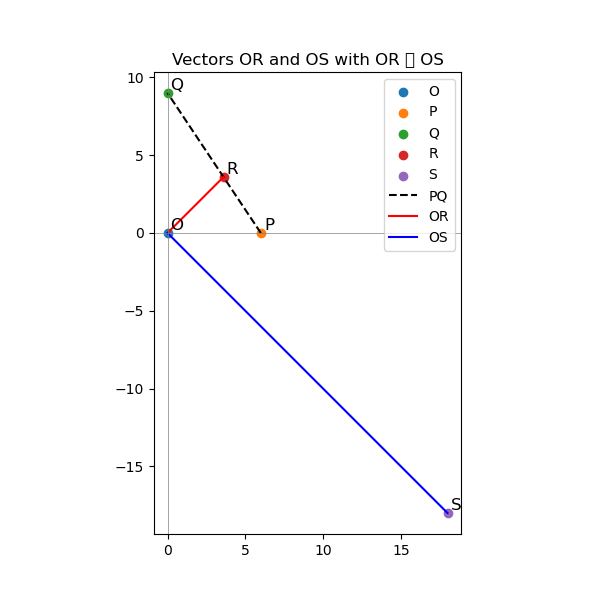
\includegraphics[width=1.0\columnwidth]{figs/fig1.png}
    \caption{Figure for 2.10.32}
    \label{fig1}
\end{figure}

\end{document}
